\documentclass{standalone}
\usepackage{tikz}
\usetikzlibrary{shapes,arrows,positioning,calc,fit,backgrounds,shadows}

\begin{document}
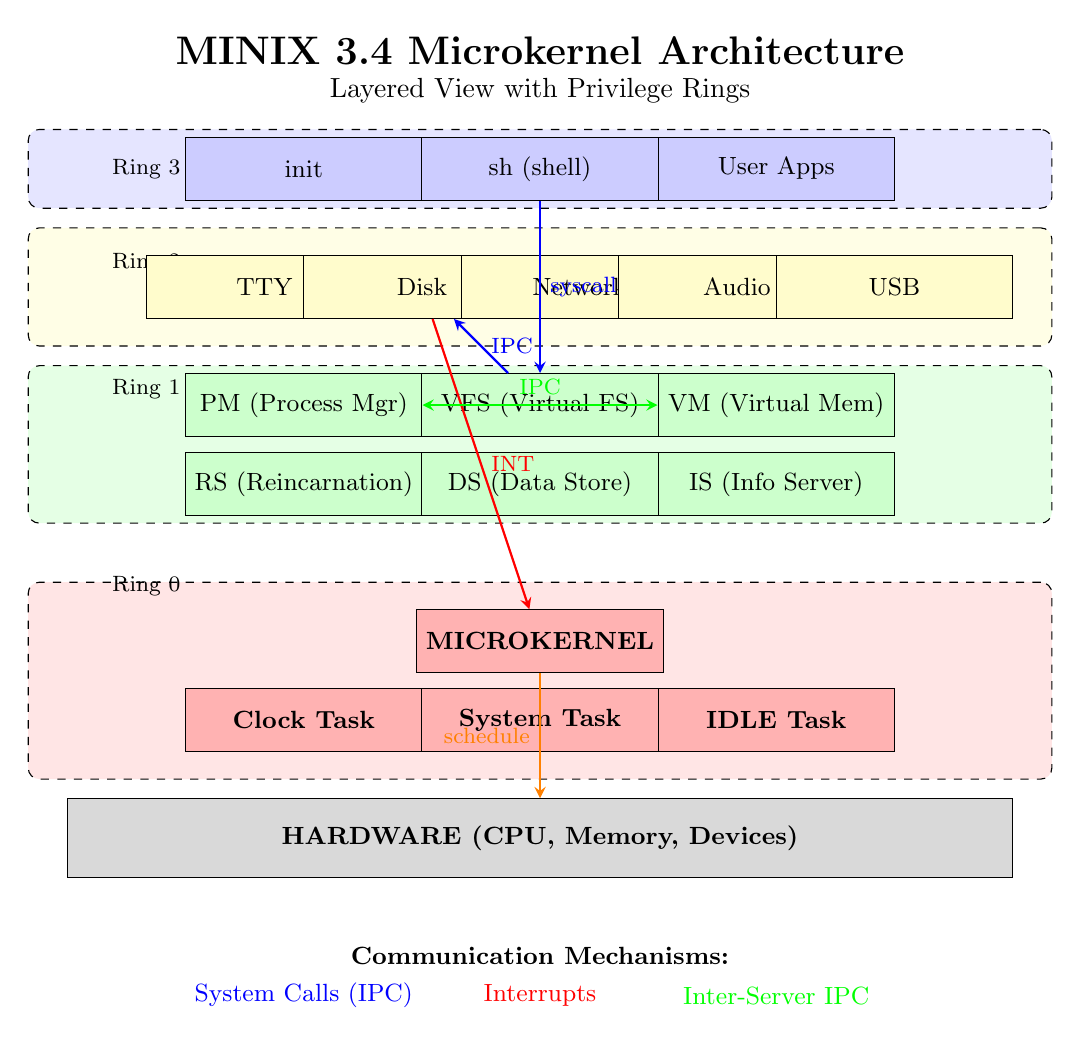
\begin{tikzpicture}[
    node distance=0.5cm,
    process/.style={rectangle, draw=black, fill=blue!20, minimum width=3cm, minimum height=0.8cm, font=\small},
    kernel/.style={rectangle, draw=black, fill=red!30, minimum width=3cm, minimum height=0.8cm, font=\small\bfseries},
    server/.style={rectangle, draw=black, fill=green!20, minimum width=3cm, minimum height=0.8cm, font=\small},
    driver/.style={rectangle, draw=black, fill=yellow!20, minimum width=3cm, minimum height=0.8cm, font=\small},
    hardware/.style={rectangle, draw=black, fill=gray!30, minimum width=12cm, minimum height=1cm, font=\small\bfseries},
    ring/.style={draw=black, dashed, rounded corners},
    arrow/.style={->, >=stealth, thick},
    bidir/.style={<->, >=stealth, thick},
    label/.style={font=\footnotesize}
]

% Title
\node[font=\Large\bfseries] at (6, 10) {MINIX 3.4 Microkernel Architecture};
\node[font=\normalsize] at (6, 9.5) {Layered View with Privilege Rings};

% Hardware layer
\node[hardware] (hw) at (6, 0) {HARDWARE (CPU, Memory, Devices)};

% Ring 0 - Kernel layer
\begin{scope}[on background layer]
    \node[ring, fill=red!10, minimum width=13cm, minimum height=2.5cm] (ring0) at (6, 2) {};
\end{scope}
\node[label] at (1, 3.2) {Ring 0};
\node[kernel] (kernel) at (6, 2.5) {MICROKERNEL};
\node[kernel] (clock) at (3, 1.5) {Clock Task};
\node[kernel] (system) at (6, 1.5) {System Task};
\node[kernel] (idle) at (9, 1.5) {IDLE Task};

% Ring 1 - System Servers
\begin{scope}[on background layer]
    \node[ring, fill=green!10, minimum width=13cm, minimum height=2cm] (ring1) at (6, 5) {};
\end{scope}
\node[label] at (1, 5.7) {Ring 1};
\node[server] (pm) at (3, 5.5) {PM (Process Mgr)};
\node[server] (vfs) at (6, 5.5) {VFS (Virtual FS)};
\node[server] (vm) at (9, 5.5) {VM (Virtual Mem)};
\node[server] (rs) at (3, 4.5) {RS (Reincarnation)};
\node[server] (ds) at (6, 4.5) {DS (Data Store)};
\node[server] (is) at (9, 4.5) {IS (Info Server)};

% Ring 2 - Device Drivers
\begin{scope}[on background layer]
    \node[ring, fill=yellow!10, minimum width=13cm, minimum height=1.5cm] (ring2) at (6, 7) {};
\end{scope}
\node[label] at (1, 7.3) {Ring 2};
\node[driver] (tty) at (2.5, 7) {TTY};
\node[driver] (disk) at (4.5, 7) {Disk};
\node[driver] (net) at (6.5, 7) {Network};
\node[driver] (audio) at (8.5, 7) {Audio};
\node[driver] (usb) at (10.5, 7) {USB};

% Ring 3 - User Applications
\begin{scope}[on background layer]
    \node[ring, fill=blue!10, minimum width=13cm, minimum height=1cm] (ring3) at (6, 8.5) {};
\end{scope}
\node[label] at (1, 8.5) {Ring 3};
\node[process] (init) at (3, 8.5) {init};
\node[process] (shell) at (6, 8.5) {sh (shell)};
\node[process] (user) at (9, 8.5) {User Apps};

% IPC arrows
\draw[arrow, blue] (shell) -- node[right, label] {syscall} (vfs);
\draw[arrow, blue] (vfs) -- node[right, label] {IPC} (disk);
\draw[arrow, red] (disk) -- node[right, label] {INT} (kernel);
\draw[bidir, green] (pm) -- node[above, label] {IPC} (vm);
\draw[arrow, orange] (kernel) -- node[left, label] {schedule} (hw);

% Legend
\node[font=\small\bfseries] at (6, -1.5) {Communication Mechanisms:};
\node[font=\small, blue] at (3, -2) {System Calls (IPC)};
\node[font=\small, red] at (6, -2) {Interrupts};
\node[font=\small, green] at (9, -2) {Inter-Server IPC};

\end{tikzpicture}
\end{document}